\section{Methodology}
\subsection{Strategy}
Streaming systems are typically evaluated by two major metrics:
\begin{itemize}
\item \textbf{Throughput:} We evaluate throughput as the number of tuples that a full system is capable of processing per second.
\item \textbf{Latency:} We consider latency numbers to be the period of time between a tuple's generation and when it is fully processed by the streaming system.  The latency number that a window reports each reporting interval is the current time minus the timestamp of its oldest tuple.
\end{itemize}

In both of the benchmarks we use in our comparisons, we consider a tuple to be string of text of a fixed number of words, the first of which indicates the tuple's epoch timestamp in milliseconds.  We then append a second timestamp to the tuple at the end of processing.  We calculate our latency by subtracking our initial timestamp from our final timestamp.  We calculate our throughput by counting the number of tuples with an initial timestamp that are processed within the given window of time.

\subsection{Architecture Philosophy}
A typical streaming system recieves new tuples of data from an outside source via some external connection.  The system then processes the data, stores information as necessary, and then outputs results as another stream to be displayed or used by other applications.  We are only interested in evaluating the stream processing portion of this process.

When benchmarking specific workloads, we intended to put as little external strain on the system as possible in order to avoid contaminating our results.  The actual streaming system is hosted on a specific number of machines, with separate machines generating tuples and sending them via the network.  In addition, the output is also sent to yet another machine and written to disk there, again minimizing extra strain on the machines actually performing the workload.

\john{INSERT DIAGRAM OF INTENDED BENCHMARKING STRATEGY HERE}

\subsection{Benchmarks}
We evaluated our systems using two workloads: Wordcount and Grep

\subsubsection{Wordcount}
In the Wordcount benchmark, each input tuple is broken down into individual words and counted within a window of time.  This benchmark should favor Spark, as it is highly parallelizeable.   Spark breaks these tuples into an array of words and then performs map and reduce operations to find their counts.  System-X on the other hand must iterate over each tuple, generate a new tuple for each word, and then perform an aggregation on the resulting tuples.

\john{Insert diagram of each benchmark, one from Spark perspective one for System-X}

\subsubsection{Grep}
In the Grep benchmark, input tuples are sent through a filter operation in order to find sentences which contain the word "the."  Both Spark and System-X execute similar strategies for this benchmark.

\begin{figure}[t]
\centering
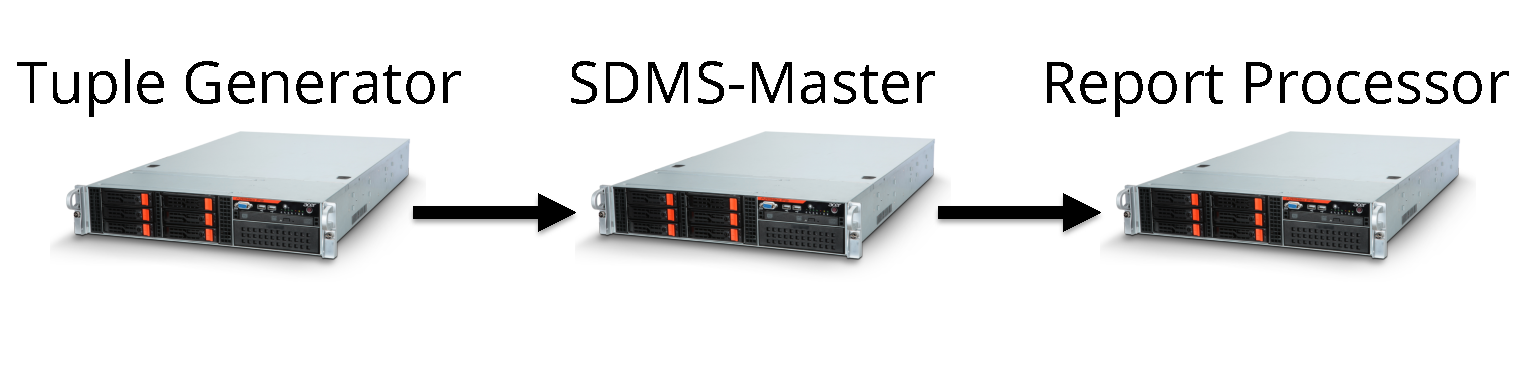
\includegraphics[width=1\linewidth]{figures/diagram.pdf}
%\vspace{-0.3in}
\caption{setup}
\label{fig:sb1-tput}
\end{figure}

\begin{figure}[t]
\centering
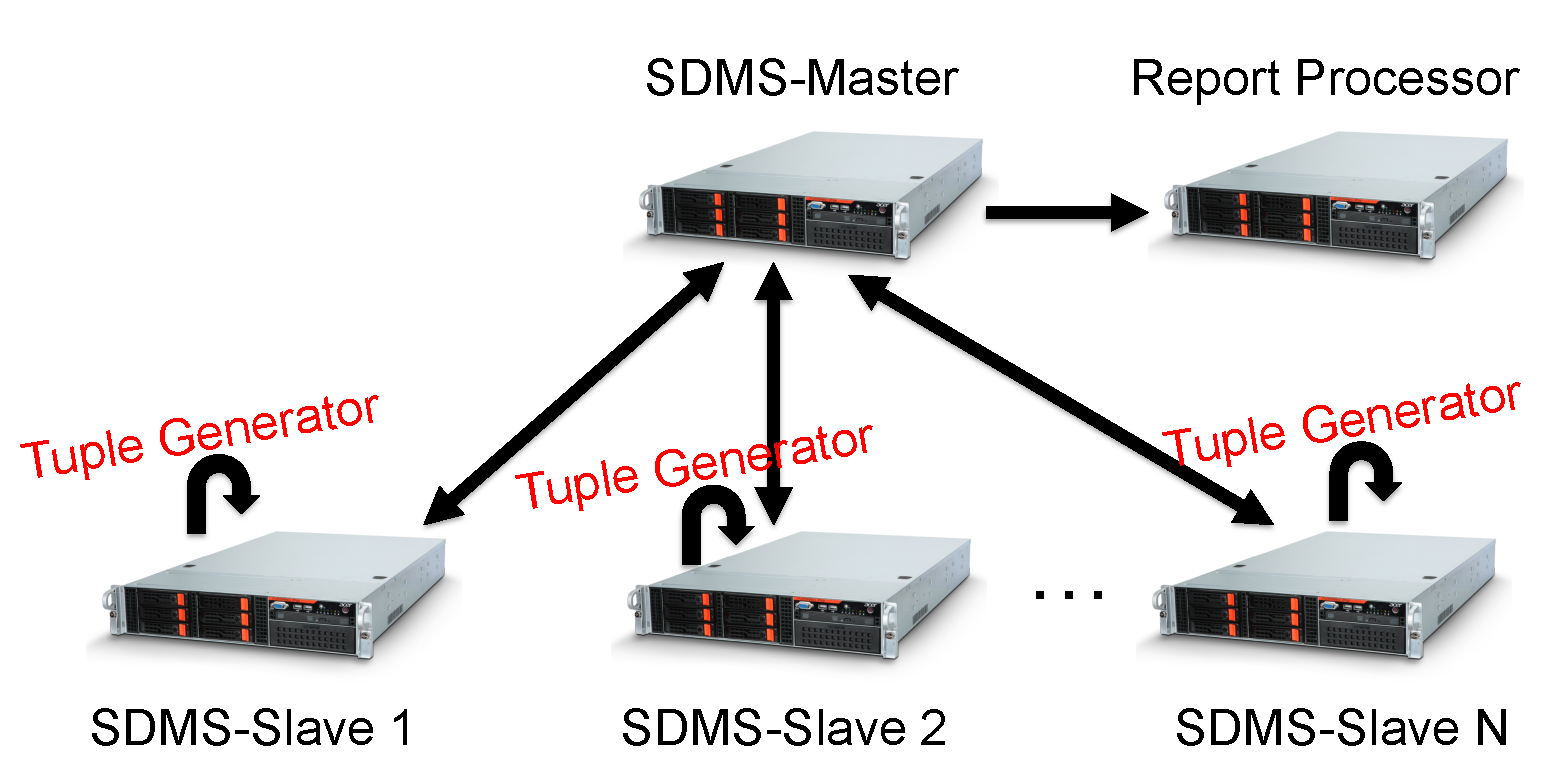
\includegraphics[width=1\linewidth]{figures/spark-full-diagram.pdf}
%\vspace{-0.3in}
\caption{setup, full spark}
\label{fig:sb1-tput}
\end{figure}



